\documentclass[10pt,twocolumn,letterpaper]{article}

\usepackage{dependable_dnn}
\usepackage{times}
\usepackage{epsfig}
\usepackage{graphicx}
\usepackage{amsmath}
\usepackage{amssymb}
\usepackage{subfigure}
\usepackage[table, dvipsnames]{xcolor}

% Include other packages here, before hyperref.

% If you comment hyperref and then uncomment it, you should delete
% egpaper.aux before re-running latex.  (Or just hit 'q' on the first latex
% run, let it finish, and you should be clear).
\usepackage[pagebackref=true,breaklinks=true,letterpaper=true,colorlinks,bookmarks=false]{hyperref}

\iccvfinalcopy % *** Uncomment this line for the final submission

\def\iccvPaperID{} % *** Enter the Paper ID here
\def\httilde{\mbox{\tt\raisebox{-.5ex}{\symbol{126}}}}

% Pages are numbered in submission mode, and unnumbered in camera-ready
\ificcvfinal\pagestyle{empty}\fi

\begin{document}

%%%%%%%%% TITLE - PLEASE UPDATE
\title{Ask Not What AI Can Do, But What AI Should Do: Towards a Framework of Task Delegability \\ {\rm {\normalsize Seungmin Lee (profile2697@gmail.com; 2013-11420), Dept. of Computer Science and Engineering, Seoul National University}}}   % **** Enter the paper title and student information here

\maketitle
\thispagestyle{empty}

%%%%%%%%% BODY TEXT - ENTER YOUR RESPONSE BELOW

%%%%%%%%%%%%%%%%%
%%%%%%%%%%%%%%%%%
\section{Motivation of This Work}
The recent development of artificial intelligence (AI) has made people look forward to the opportunities that the technology will bring to us. At the same time, however, there is growing concerns about which tasks and to what extent AI should be applied. These concerns can be naturally rewritten as a following question: Which tasks can be delegated to AI? 

According to the paper, there is two dimensions that should be considered to answering the question. The first dimension is \textit{what AI can do}, or \textit{capability}. This means performance of AI for a particular task. Almost all traditional researches are about this dimension. The second dimension is \textit{what AI should do}, or \textit{human preference} which means what role human wants to delegate to AI. This is clearly important dimension, but virtually no research has been conducted. This work is the first empirical study about the second dimension and has been conducted for better understanding of how different factors affect human preferences of delegation (\textit{delegability}). 

\section{Approach}
For this work, the authors have done following three steps: devising a framework based on four factors that are considered to affect the delegability, constructing a dataset of diverse tasks like 'dignosing cancers' for understanding the delegabilities in different tasks, conducting a survey created using the factors and dataset to investigate how much AI's involvement is preferred by people. 

\subsection{Step 1: Devising a Framework for Delegability}
\paragraph{Four Factors}
The authors devised a framework with four high-level factors considered to affect delegability: a person's \textbf{motivation}, task's \textbf{difficulty}, a person's subjective perception of \textbf{risk} that the one should take, and a person's \textbf{trust} in AI agent. These factors are further divided into sub-concepts as shown in Table~\ref{tab:four_factors}.


\paragraph{Delegability}
The authors splited degree of delegation to measure human preferences according to the four factors. It is splited into the follwing four levels: \textbf{No AI assistance}, \textbf{The human leads and the AI assists} (or \textit{machine-in-the-loop}), \textbf{The AI leads and the human assists} (or \textit{human-in-the-loop}) and \textbf{Full AI automation}.

\subsection{Step 2: Constructing a Dataset of 100 Tasks}
To evaluate the framework empirically, the authors collected diverse tasks from academic conferences, media, well-known occupations and people's everyday-life such as 'Identifying fake news article'(from conferences) or 'buying a birthday present'(from everday-life).


\subsection{Step 3: Conducting a Survey}
The authors conducted 5-minute survey using Amazon Mechanical Turk. They used two versions of survey: \textbf{Personal Survey} and \textbf{Expert Survey} because if a subject does not perform a task that requires expertise, e.g., 'diagnosing cancer', the motivation can not be estimated. They recorded total 1000 responses:  500 personal and expert surveys each and 5 for the 100 tasks each.
\vspace{0.2cm}

\section{Results}
On both personal and expert surveys, the subjects prefer \textit{machine-in-the-loop}, and have little preference for \textit{AI only} as we can see on Figure~\ref{fig:dist}. Examining the correlation between the delegability and the four factors, trust showed the strongest correlation. However, interestingly, interpretability which belongs to sub-concepts of trust does not show significant relationships. They also investigated relations between factors and found difficulty and risk have the strongest correlation. Additionally, the authors trained a classifier for verfifying the proposed framework and the classifier shows better performance than a random baseline.


\begin{figure}[b]
	\centering
	\subfigure[Individual preferences.]{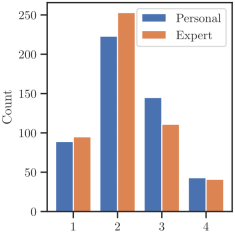
\includegraphics[width=4cm, height=2.5cm]{assets/hist_cmp_label.png}}
	\subfigure[Averaged preferences for each task.]{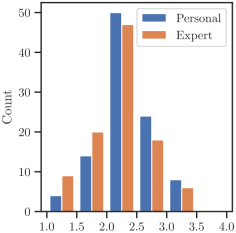
\includegraphics[width=4cm, height=2.5cm]{assets/hist_cmp_label_flattened.png}}
	\caption{Distributions of survey responses. 1 is Human only, and 4 is AI only}
	\label{fig:dist}
\end{figure}


{\small
\bibliographystyle{ieee}
%\bibliography{egbib}
}


\begin{table}[t]
	\centering
	\resizebox{0.48\textwidth}{!}{
		\begin{tabular}{l l}	
			\hline\hline
			\textbf{Factors} & \textbf{Components} \\
			\hline
			Motivation  & Intrinsic motivation, goals, utility \\
			\hline
			Difficulty &  Social skills, creativity, effort required, expertise required, human ability \\
			\hline
			Risk & Accountability, uncertainty, impact  \\
			\hline
			Trust& Machine ability, interpretability, value alignment\\
			\hline\hline
	\end{tabular}}
	\caption{
		An overview of the four factors in the framework.
	}\label{tab:four_factors}
\end{table}

\end{document}
